\chapter{Results}
\label{chap:results}

The evaluation has two phases. \textbf{Phase~1} measures the model itself on ground-truth vehicle boxes with controlled occlusions, under the pre-registered protocol (thresholds on validation, a single locked test run). \textbf{Phase~2} measures how much of that advantage survives in a realistic deployment, where boxes come from a live YOLOv8n detector and occlusions are natural. All numbers below are read from frozen result files (\texttt{release/FROZEN\_RESULTS.md}); 95\% confidence intervals are paired bootstrap intervals with the camera \emph{location} as resampling unit ($15$ test locations, $10{,}000$ draws).

\section{Data Preprocessing}
\label{sec:data_preprocessing}

Static \texttt{ignored} regions ($528{,}798$ rows, $407$ polygons) were separated from vehicle annotations, and $72{,}714$ vehicle boxes ($5.7\%$) whose centres fall inside them were removed, leaving $1{,}201{,}341$ boxes in $8{,}251$ trajectories. Fixed event sets were generated once and hashed: $6{,}000$ validation events ($11{,}389$ lost tracks) and $12{,}000$ test events ($27{,}120$ lost tracks). Because the official test split shares $7$ of its $15$ camera locations with train/validation, the test set was also scored separately on shared and unseen locations: GapLink-Lite reaches $93.39\%$ and $93.44\%$ Top-1 respectively (C-3: $80.59\%$ and $79.96\%$), so performance does not depend on having seen the camera.

\section{Exploratory Data Analysis (EDA)}
\label{sec:eda}

Figure~\ref{fig:eda_results} shows the trajectory-length and traffic-density distributions together with median backgrounds of the $25$ camera clusters used for the location-disjoint split. Traffic is dense (mean $8.7$ vehicles per frame; $45{,}603$ frames with $\ge 10$ vehicles), which makes nearby look-alike candidates the main source of wrong links. Training converges within $2{,}400$ steps (about $100$~s per run on an RTX~3050; Figure~\ref{fig:training_curves}).

\begin{figure}[htbp]
    \centering
    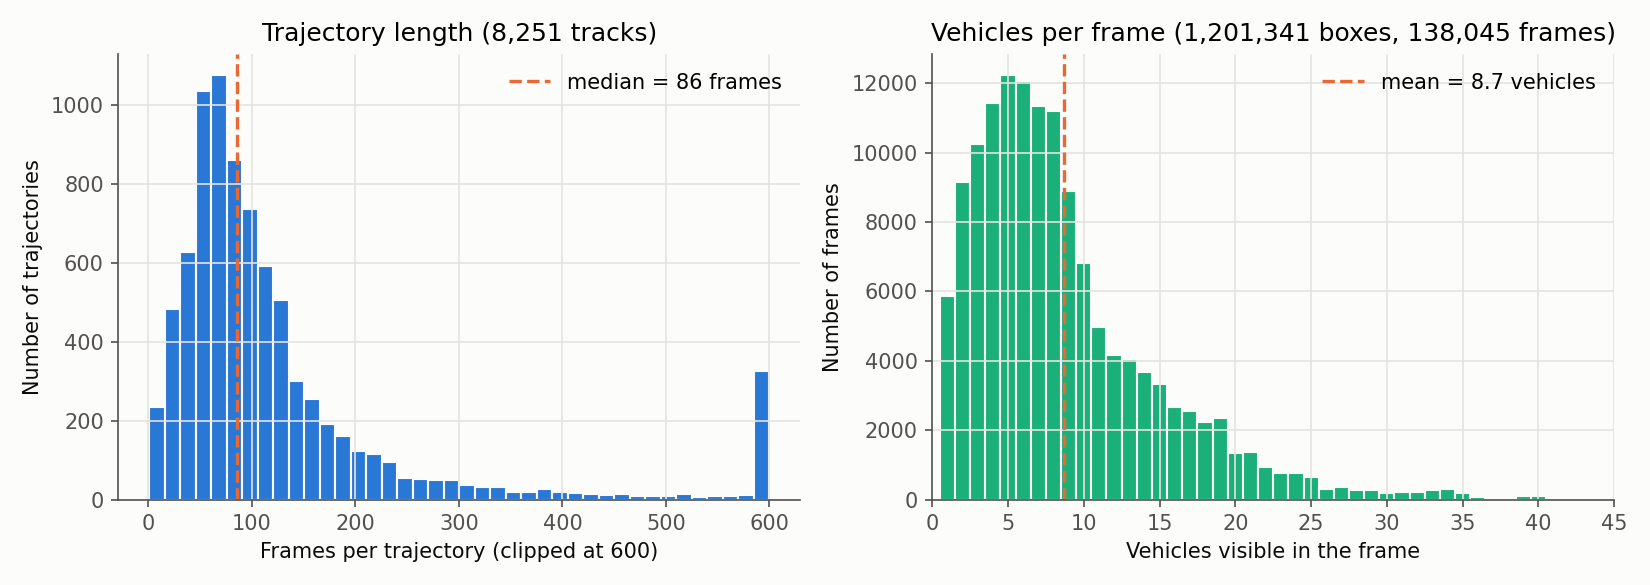
\includegraphics[width=0.52\textwidth]{figures/fig_class_hist.png}\hfill
    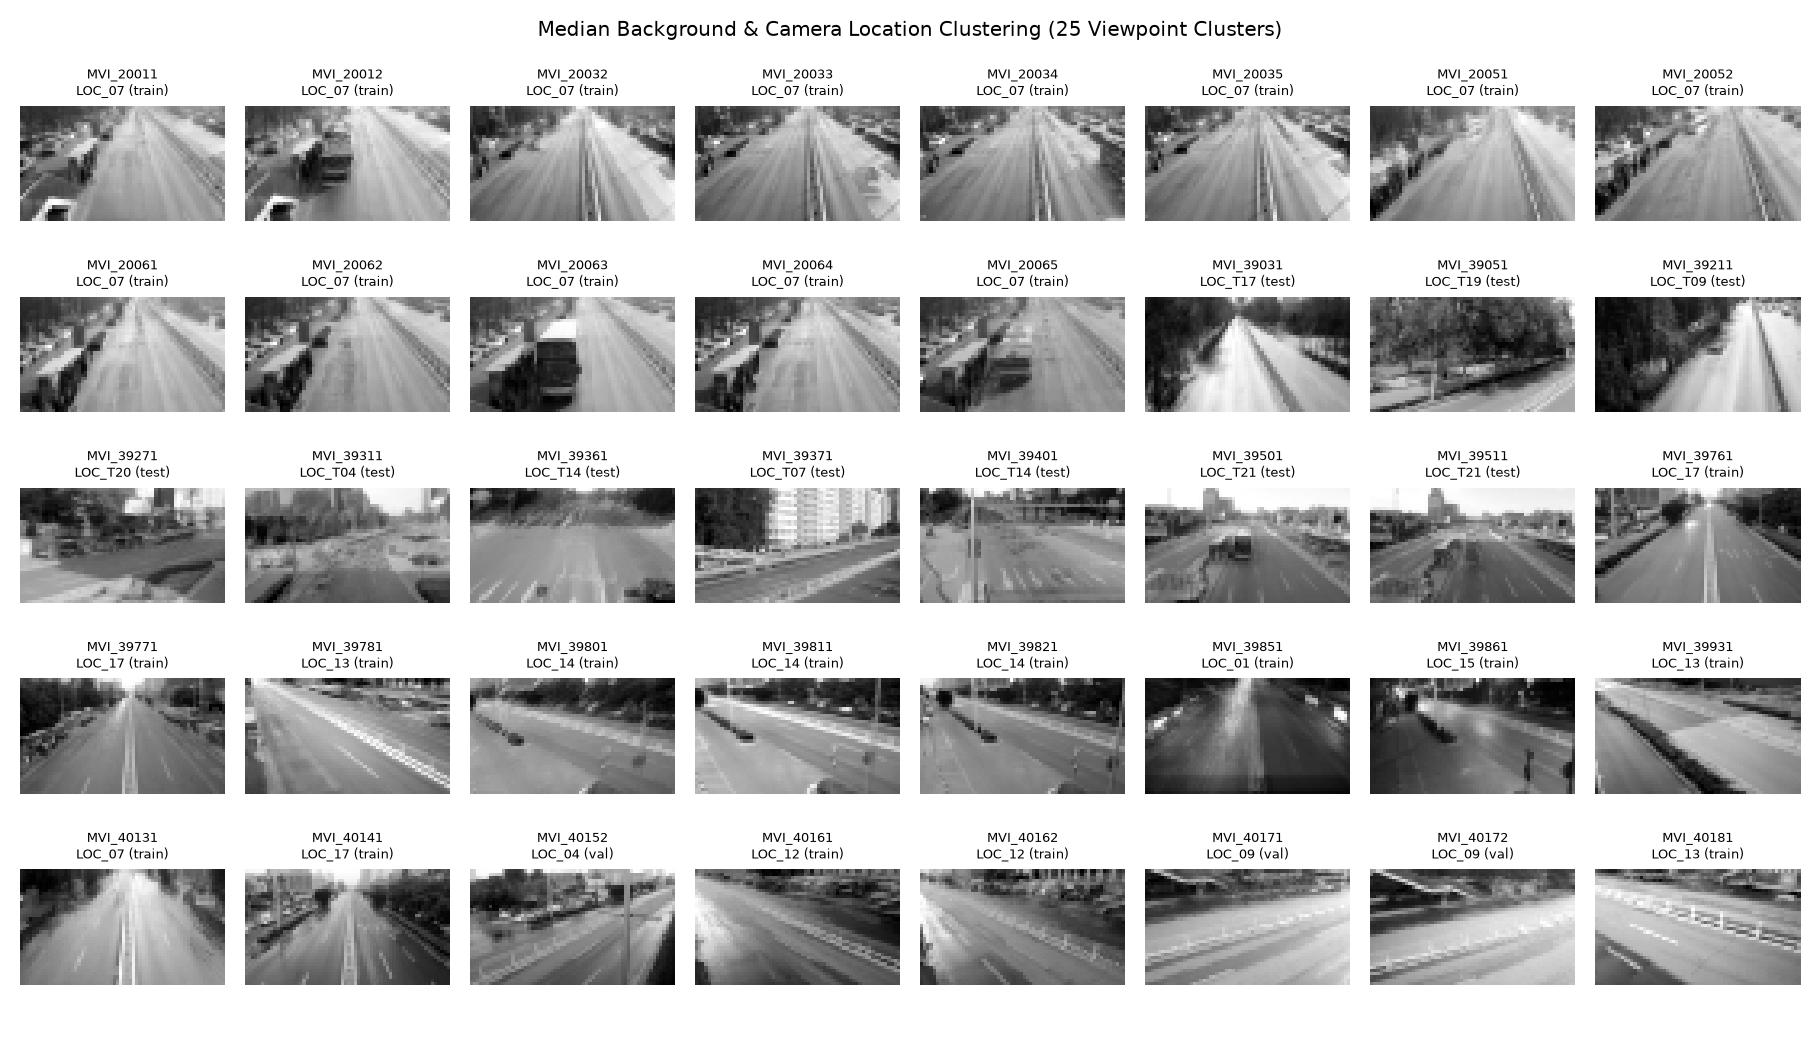
\includegraphics[width=0.46\textwidth]{figures/fig_location_clusters.png}
    \caption{Exploratory Data Analysis: Trajectory Length \& Density (left) and 40 Representative Median Backgrounds Across 25 Raw Camera Clusters (right)}
    \label{fig:eda_results}
\end{figure}

\begin{figure}[htbp]
    \centering
    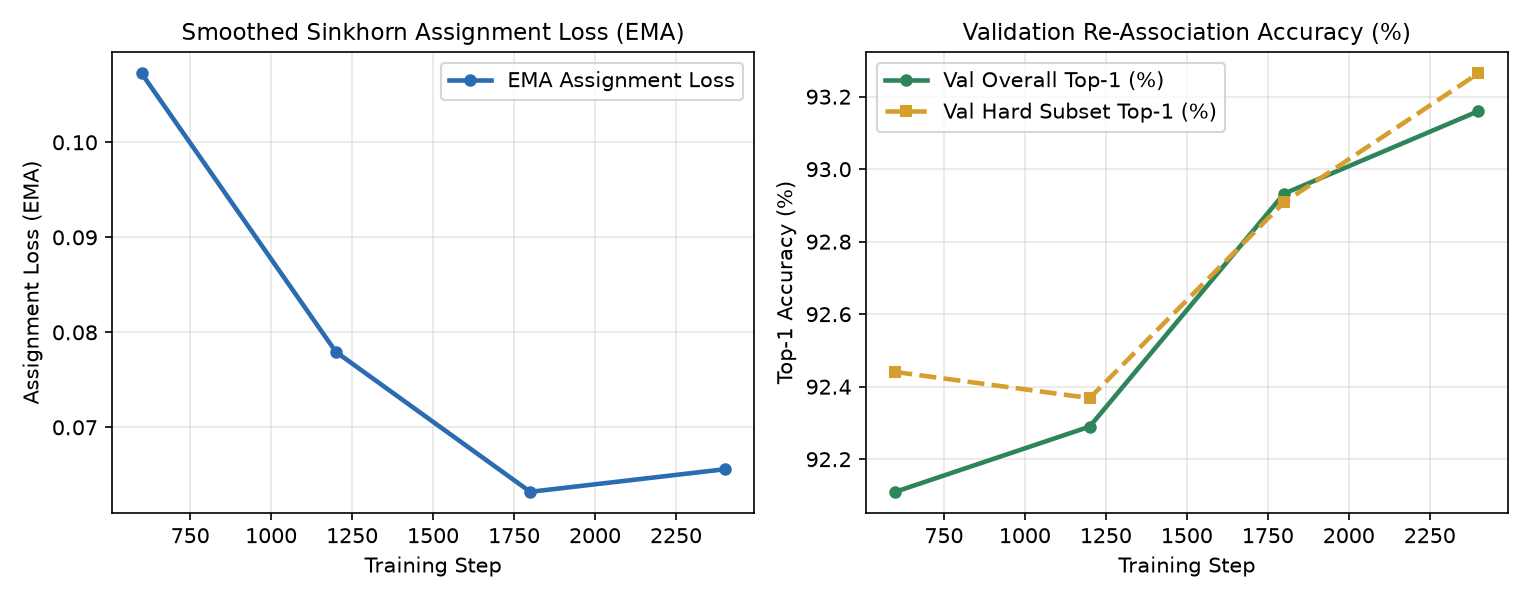
\includegraphics[width=0.95\textwidth]{figures/fig_training_curves.png}
    \caption{GapLink-Lite Convergence: Smoothed EMA Assignment Loss (left) and Validation Top-1 Accuracy (right)}
    \label{fig:training_curves}
\end{figure}

\section{Modeling}
\label{sec:modeling}

\subsection{Phase 1: Controlled Evaluation on Ground-Truth Boxes}
\label{sec:phase1}

\textbf{Event-level re-association.} Table~\ref{tab:event_results} compares the frozen checkpoint with the three classical baselines at their validation-selected thresholds. GapLink-Lite reaches $\mathbf{93.41\%}$ Top-1 with $\mathbf{3.01\%}$ wrong links (5-seed mean $93.64\% \pm 0.14\%$), against $80.29\%$ / $19.24\%$ for the Kalman baseline C-3 and $83.69\%$ / $15.88\%$ for the strongest baseline C-4. The gain is $+13.12$~pp over C-3 (95\% CI $[12.29, 14.19]$) and $+9.72$~pp over C-4 ($[8.68, 10.94]$), and it is largest where classical motion models break down: on long gaps ($46$--$90$ frames) Top-1 rises from $64.24\%$ (C-4) to $79.58\%$. Figure~\ref{fig:wlr_curve} shows that this is not an artefact of threshold choice: over the full threshold range, GapLink-Lite's curve lies above every baseline curve.

\begin{table}[htbp]
    \centering
    \caption{Phase 1 --- event-level re-association on the locked test split ($12{,}000$ events, $27{,}120$ lost tracks). All thresholds selected on validation.}
    \label{tab:event_results}
    \scriptsize\setlength{\tabcolsep}{2.8pt}
    \begin{tabularx}{\textwidth}{X c c c c c c c}
        \toprule
        \textbf{Method (Op. Point)} & \textbf{Top-1 (\%)} & \textbf{Short} & \textbf{Med} & \textbf{Long} & \textbf{Hard (\%)} & \textbf{Dust F1} & \textbf{WLR (\%)} \\
        \midrule
        C-2 (Best Val Top-1) & 76.58 & 87.80 & 76.64 & 49.10 & 77.73 & 44.77 & 21.14 \\
        C-3 (Best Val Top-1) & 80.29 & 94.23 & 76.74 & 54.39 & 81.70 & 52.31 & 19.24 \\
        C-4 (Best Val Top-1) & 83.69 & 94.41 & 80.77 & 64.24 & 85.85 & 51.22 & 15.88 \\
        \midrule
        C-2 (Val WLR$\le$5\%) & 70.59 & 93.82 & 63.88 & 29.32 & 69.67 & 49.41 & 6.46 \\
        C-3 (Val WLR$\le$5\%, $\theta=0.5$) & 57.22 & 46.68 & 68.79 & 56.54 & 55.76 & 39.40 & 9.13 \\
        C-4 (Val WLR$\le$5\%) & 76.03 & 74.02 & 82.25 & 66.79 & 75.89 & 54.01 & 6.70 \\
        \midrule
        \textbf{GapLink-Lite (Seed 1)} & \textbf{93.41} & \textbf{98.64} & \textbf{93.89} & \textbf{79.58} & \textbf{93.18} & \textbf{83.97} & \textbf{3.01} \\
        \textbf{GapLink-Lite (5-Seed Mean)} & \textbf{93.64} & \textbf{98.46} & \textbf{94.17} & \textbf{80.67} & \textbf{93.47} & \textbf{84.61} & \textbf{2.98} \\
        \bottomrule
    \end{tabularx}
\end{table}

\begin{figure}[htbp]
    \centering
    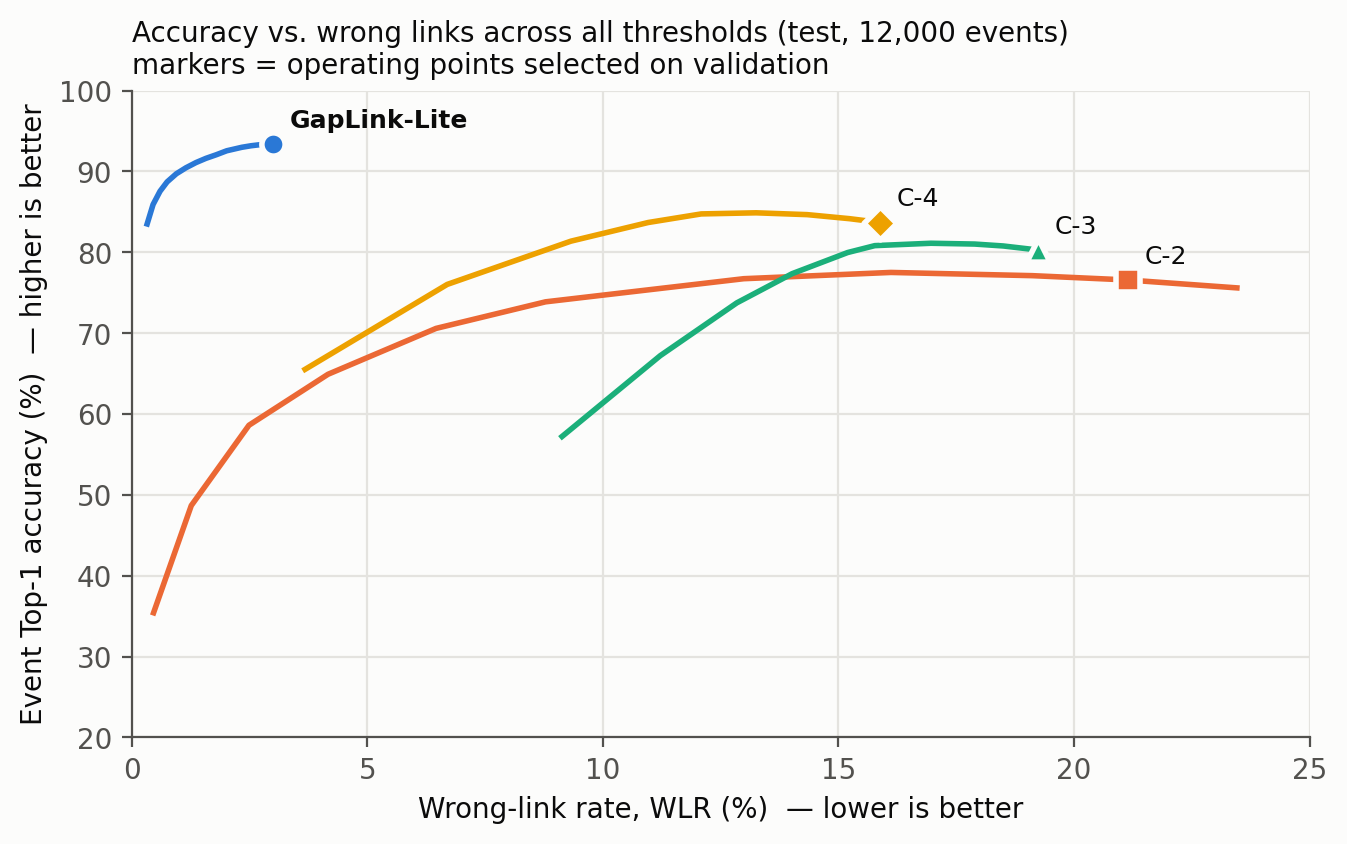
\includegraphics[width=0.86\textwidth]{figures/fig_top1_vs_wlr_curve.png}
    \caption{Event Top-1 accuracy vs.\ wrong-link rate over the full threshold range (test). Markers: validation-selected operating points.}
    \label{fig:wlr_curve}
\end{figure}

\begin{figure}[htbp]
    \centering
    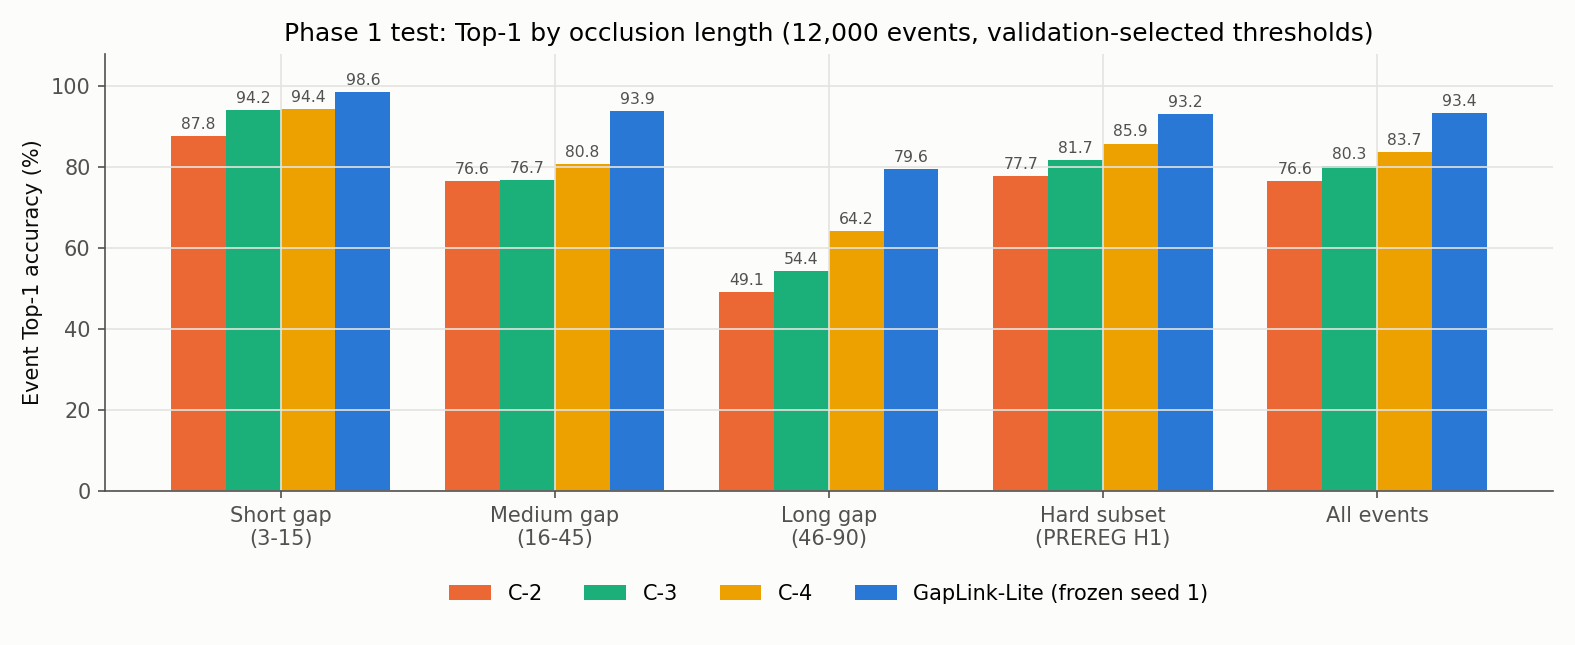
\includegraphics[width=0.95\textwidth]{figures/fig_event_gap_bins.png}
    \caption{Test Event-Level Top-1 Accuracy Across Occlusion Gap Bins and Strict Proximity ($<0.5h$)}
    \label{fig:event_gap_bins}
\end{figure}

\textbf{Uncertainty calibration (H2).} The pre-registered criterion requires calibrated 90\% coverage within $[85, 95]\%$ in all three gap bins. Short and medium gaps meet it, but the long-gap bin over-covers slightly ($95.14\%$ on validation, $95.86\%$ on test), so \textbf{H2 is not supported}. The cause is the long-gap scale factor fitted on only four validation locations. The raw Gaussian head is already close to calibrated (test: $86.42\% / 85.46\% / 88.02\%$) and is far sharper than the Kalman baseline, whose ellipses over-cover at $\approx 98\%$ with higher NLL ($9.15$ vs.\ $7.99$ px); we report this as a post-hoc observation, not as a passed hypothesis.

\begin{table}[htbp]
    \centering
    \caption{Empirical 90\% ellipse coverage and 2D NLL (H2 band $[85, 95]\%$; bold = outside band)}
    \label{tab:calib_results}
    \small\setlength{\tabcolsep}{3.5pt}
    \begin{tabularx}{\textwidth}{X c c c c c}
        \toprule
        \textbf{Model / Uncertainty State} & \textbf{Overall Cov90 (\%)} & \textbf{Short (3-15)} & \textbf{Med (16-45)} & \textbf{Long (46-90)} & \textbf{2D NLL (px) $\downarrow$} \\
        \midrule
        C-3 (Kalman Baseline) & 97.79 & 97.68 & 97.72 & 98.23 & 9.15 \\
        \textbf{GapLink-Lite, post-calib, Validation (PREREG H2)} & 88.27 & 87.71 & 87.64 & \textbf{95.14} & 8.36 \\
        \textbf{GapLink-Lite, post-calib, Test} & 90.22 & 87.87 & 90.26 & \textbf{95.86} & 8.00 \\
        \midrule
        GapLink-Lite, uncalibrated, Test (post-hoc) & 86.32 & 86.42 & 85.46 & 88.02 & 7.99 \\
        GapLink-Lite, uncalibrated, Test, 5-seed (post-hoc) & $86.83\pm0.50$ & $86.90\pm0.80$ & $85.97\pm0.76$ & $88.64\pm1.24$ & $\mathbf{7.93\pm0.18}$ \\
        \bottomrule
    \end{tabularx}
\end{table}

\begin{figure}[htbp]
    \centering
    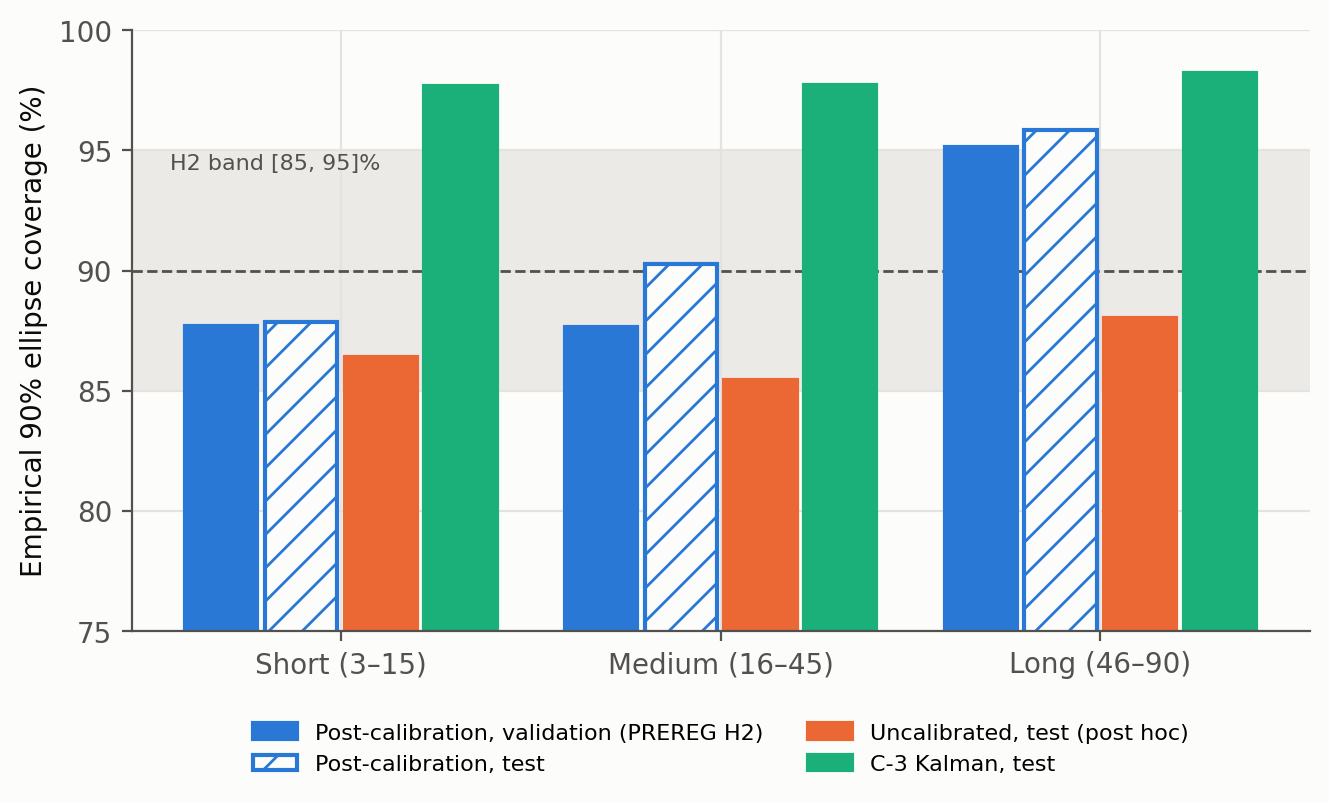
\includegraphics[width=0.86\textwidth]{figures/fig_calibration_coverage.png}
    \caption{Empirical 90\% ellipse coverage per gap bin; shaded band = H2 target $[85, 95]\%$.}
    \label{fig:calib_plot}
\end{figure}

\textbf{Online tracking (H3, P1).} Inside the two-stage online tracker (Table~\ref{tab:tracker_results}), GapLink-Lite recovers $\mathbf{96.20\%}$ of injected occlusions with only $\mathbf{0.21\%}$ wrong links, versus $85.17\%$ / $4.32\%$ for C-2 and $84.96\%$ / $10.25\%$ for C-3; IDF1 rises from $77.60\%$ (C-3) to $\mathbf{99.11\%}$ and identity switches fall from $342$ to $98$. The IRR gain over C-3 is $+11.24$~pp (CI $[9.10, 14.35]$), and GapLink-Lite beats both C-2 and C-3 in all three gap bins, so \textbf{H3 is supported}. Under partial occlusion with visible-crop appearance only, the result holds ($95.99\%$ IRR, $0.36\%$ WLR). The protocol check \textbf{P1 passes}: without re-association (C-1) IRR is $0.00\%$. All pre-registered outcomes are summarised in Section~\ref{sec:motivation_objective}.

\begin{table}[htbp]
    \centering
    \caption{Phase 1 --- online tracker on $40$ test sequences ($1{,}922$ injected occlusion intervals, $a_{\max}=95$)}
    \label{tab:tracker_results}
    \resizebox{\textwidth}{!}{%
    \begin{tabular}{@{}l rrrrrrrrr@{}}
        \toprule
        \textbf{Tracker} & \shortstack{\textbf{Full}\\\textbf{IRR}} & \shortstack{\textbf{Full}\\\textbf{WLR}} & \shortstack{\textbf{Full}\\\textbf{IDF1}} & \shortstack{\textbf{Full}\\\textbf{MOTA}} & \shortstack{\textbf{Full}\\\textbf{IDSW}} & \shortstack{\textbf{Part}\\\textbf{IRR}} & \shortstack{\textbf{Part}\\\textbf{WLR}} & \shortstack{\textbf{Part}\\\textbf{IDF1}} & \shortstack{\textbf{Part}\\\textbf{IDSW}} \\
        \midrule
        C-1 (IoU Only) & 0.00 & 0.00 & 74.18 & 99.59 & 2127 & 0.00 & 0.00 & 74.18 & 2127 \\
        C-2 (Const-Vel) & 85.17 & 4.32 & 94.66 & 99.92 & 331 & 85.38 & 4.21 & 94.42 & 327 \\
        C-3 (Kalman) & 84.96 & 10.25 & 77.60 & 99.93 & 342 & 81.17 & 14.15 & 76.63 & 416 \\
        C-3 (WLR$\le$5\%) & 77.58 & 3.07 & 95.23 & 99.88 & 487 & 49.43 & 7.70 & 87.21 & 1029 \\
        C-4 (C-3+S+C) & 85.12 & 10.15 & 76.98 & 99.93 & 338 & 82.21 & 12.90 & 76.43 & 395 \\
        \textbf{GapLink-Lite} & \textbf{96.20} & \textbf{0.21} & \textbf{99.11} & \textbf{99.98} & \textbf{98} & \textbf{95.99} & \textbf{0.36} & \textbf{99.02} & \textbf{103} \\
        \bottomrule
    \end{tabular}%
    }
\end{table}

\begin{figure}[htbp]
    \centering
    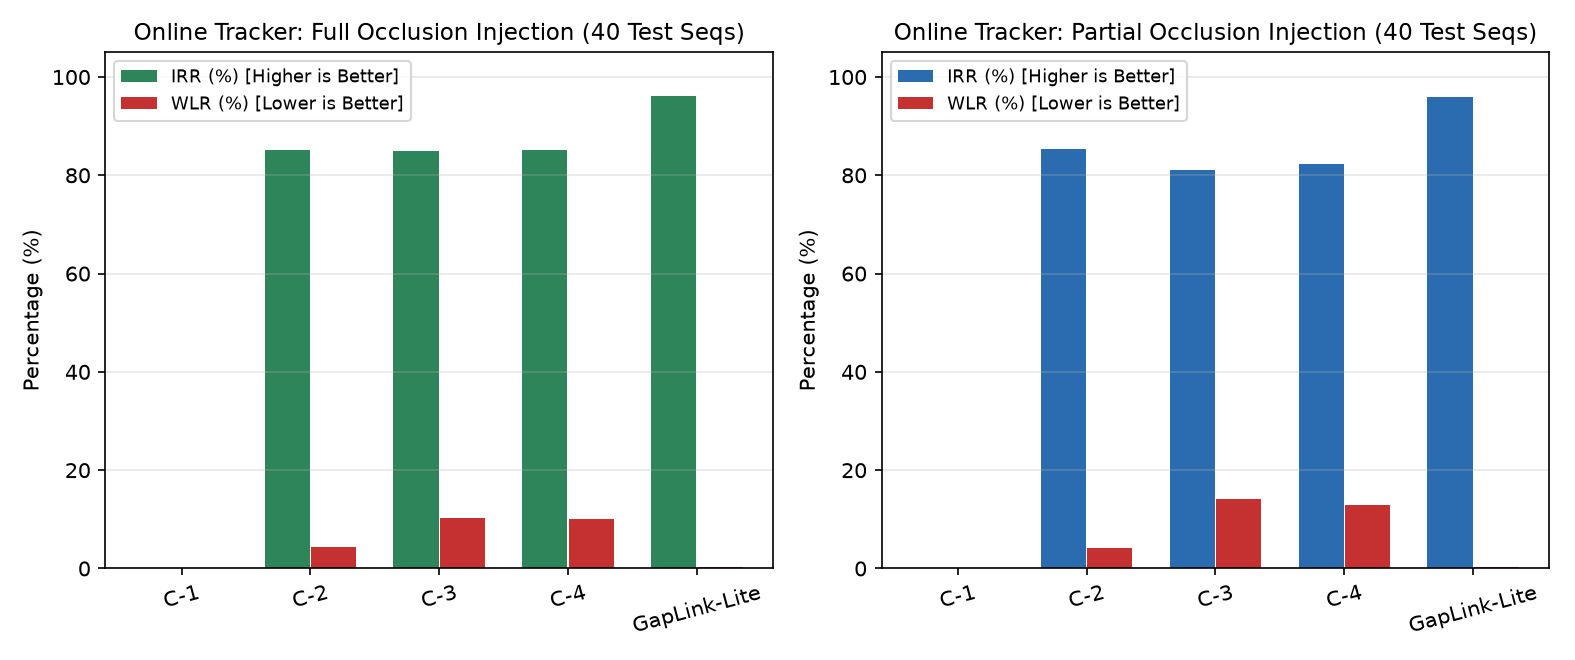
\includegraphics[width=0.95\textwidth]{figures/fig_tracker_irr_wlr.png}
    \caption{Online Tracker Identity Recovery Rate (IRR) and Wrong-Link Rate (WLR) under Full and Partial Occlusion}
    \label{fig:tracker_plot}
\end{figure}

\subsection{Phase 2: Application with a Live YOLOv8n Detector}
\label{sec:phase2}

\textbf{Setup.} All methods receive the same YOLOv8n detections (\texttt{imgsz}$=640$, confidence $0.28$) and share the same Stage-1 IoU tracker, lost-track window ($a_{\max}=95$) and security rules; only the re-association module differs. Ground truth is used solely afterwards for scoring: \emph{Nat-IRR} is the fraction of natural detector gaps ($3$--$95$ frames) after which a vehicle keeps its identity, and \emph{Nat-WLR} the fraction of re-associations that join two different vehicles. For every method the acceptance threshold was selected on the $13$ validation videos with the same rule (highest Nat-IRR subject to Nat-WLR $\le 5\%$) and evaluated once on the $40$ test videos. For this phase GapLink-Lite uses a detector-aware checkpoint (\texttt{release/live\_v1.3.pt}) fine-tuned from the frozen model on YOLOv8n events of the training sequences (Section~\ref{sec:training_methodology}).

\textbf{Choice of baselines.} Third-party trackers cannot be used under the project constraints, so each classical paradigm is represented by a self-implemented associator (Table~\ref{tab:baseline_families}).

\begin{table}[htbp]
    \centering
    \caption{Classical re-association paradigms used as baselines}
    \label{tab:baseline_families}
    \small
    \begin{tabularx}{\textwidth}{l X X}
        \toprule
        \textbf{Baseline} & \textbf{Paradigm} & \textbf{Counterpart in practice} \\
        \midrule
        C-1 & IoU matching only, no re-association & Lower bound; SORT once a track is deleted \cite{bewley2016sort} \\
        C-2 & Constant-velocity extrapolation + Hungarian & Heuristic motion trackers \\
        C-3 & Kalman filter + Mahalanobis gating & Motion model of SORT, DeepSORT, ByteTrack, OC-SORT \cite{bewley2016sort,wojke2017deepsort,zhang2022bytetrack,cao2023ocsort} \\
        C-4 & C-3 + box size + colour histogram & DeepSORT-style motion + appearance (without a ReID network) \\
        \bottomrule
    \end{tabularx}
\end{table}

\textbf{Results.} Table~\ref{tab:live_v13} and Figure~\ref{fig:live_scatter} show the outcome. Against the Kalman family that underlies industrial trackers, GapLink-Lite is better on both axes: Nat-IRR $\mathbf{84.41\%}$ vs.\ $57.63\%$ (C-3) and $61.85\%$ (C-4), Nat-WLR $\mathbf{6.09\%}$ vs.\ $24.70\%$ and $9.94\%$. Against the strongest baseline, constant velocity (C-2), recovery is equal ($84.41\%$ vs.\ $84.58\%$; $\Delta = -0.17$~pp, CI $[-1.33, 1.08]$) while \textbf{wrong links are halved} ($6.09\%$ vs.\ $12.92\%$; $\Delta = -6.82$~pp, CI $[-11.04, -3.18]$). In a security console a wrong link is a false alarm, and GapLink-Lite also has the lowest forbidden-route false-alarm rate ($9.27\%$). The detector-aware checkpoint is what makes this possible: with the original checkpoint the live wrong-link rate is $10.20\%$, and fine-tuning reduces it by $4.11$~pp (CI $[1.57, 5.98]$) at a cost of $2.89$~pp recovery.

\begin{table}[htbp]
    \centering
    \caption{Phase 2 --- live YOLOv8n evaluation with validation-selected operating points. Validation: $13$ videos; test: $40$ videos. Route metrics on occluded $Z_A\!\to\!Z_B$ crossings. $^\dagger$no threshold reached Nat-WLR $\le 5\%$ on validation (lowest-WLR rule).}
    \label{tab:live_v13}
    \resizebox{\textwidth}{!}{%
    \begin{tabular}{@{}l rr rr rr@{}}
        \toprule
        & \multicolumn{2}{c}{\textbf{Validation}} & \multicolumn{4}{c}{\textbf{Test}} \\
        \cmidrule(lr){2-3}\cmidrule(lr){4-7}
        \textbf{Method (operating point)} & \textbf{Nat-IRR} & \textbf{Nat-WLR} & \textbf{Nat-IRR} & \textbf{Nat-WLR} & \textbf{Route rec.} & \textbf{Route FAR} \\
        \midrule
        C-1 (IoU only) & 6.05 & 0.00 & 8.93 & 0.00 & 33.33 & 3.45 \\
        C-2 ($\theta=1.2$) & \textbf{81.56} & 4.87 & \textbf{84.58} & 12.92 & 41.98 & 11.32 \\
        C-3 ($\theta=1.0$)$^\dagger$ & 32.23 & 16.37 & 57.63 & 24.70 & 47.53 & 32.56 \\
        C-4 ($\theta=1.2$) & 32.08 & \textbf{3.81} & 61.85 & 9.94 & \textbf{49.38} & 14.04 \\
        GapLink-Lite v1.1 ($\tau=0.25$, reference) & 81.69 & 13.33 & 87.30 & 10.20 & 45.68 & 12.88 \\
        \textbf{GapLink-Lite v1.3} ($\tau=0.65$) & 77.55 & 4.21 & 84.41 & \textbf{6.09} & 42.59 & \textbf{9.27} \\
        \bottomrule
    \end{tabular}%
    }
\end{table}

\begin{figure}[htbp]
    \centering
    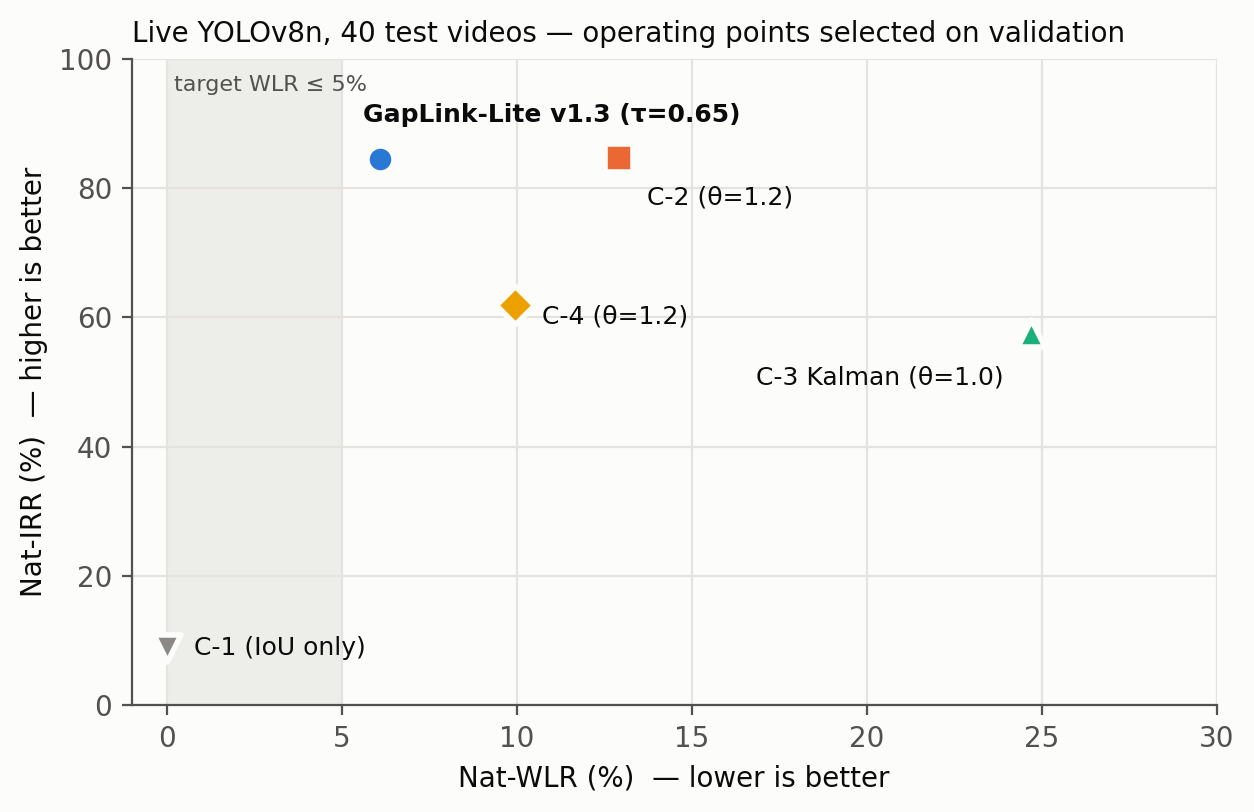
\includegraphics[width=0.78\textwidth]{figures/fig_live_v13_scatter.png}
    \caption{Phase 2 --- recovery vs.\ wrong links on $40$ live test videos (validation-selected operating points).}
    \label{fig:live_scatter}
\end{figure}

\section{User Interface}
\label{sec:user_interface}

\textbf{GapLink-VMS} (\texttt{demo/security\_vms\_app.py}) is a local web console (FastAPI) that runs YOLOv8n, the online tracker and GapLink-Lite on a video file or RTSP stream and shows a baseline and GapLink-Lite side by side (Figure~\ref{fig:vms_live_demo}). It supports three surveillance tasks: (1) forbidden routes between user-drawn zones $Z_A \to Z_B$, with entry and violation snapshots as evidence; (2) dwell-time alerts that are not reset when a passing bus hides a stopped vehicle; and (3) click-to-lock target following, which displays the predicted $2\sigma$ search region during occlusion and holds the lock (dustbin) instead of jumping to another vehicle. The baseline shown on the left can be switched between C-2, C-3 and C-4; all operating points are read from the frozen release files, and the displayed frame rate is the measured wall-clock rate. On an RTX~3050 laptop GPU the full pipeline runs at $28.95$~ms per frame ($34.5$~FPS) on a dense intersection ($12.53$~ms YOLOv8n, $3.26$~ms HSV/NMS, $13.16$~ms GapLink-Lite + VMS).

\begin{figure}[htbp]
    \centering
    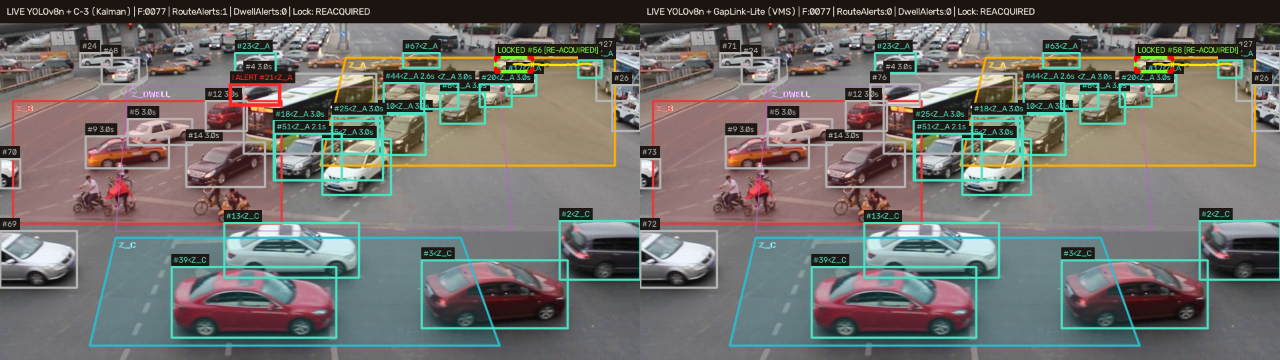
\includegraphics[width=0.96\textwidth]{figures/fig_vms_demo_intersection.png}\\[0.22cm]
    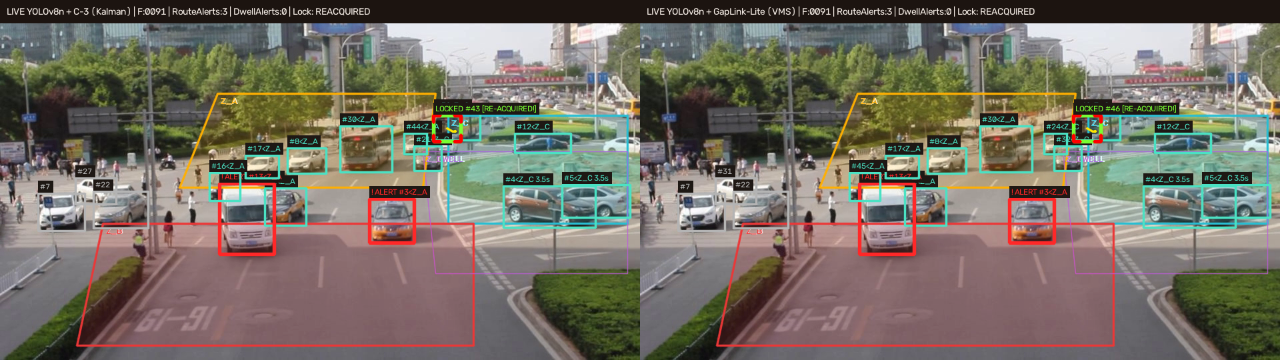
\includegraphics[width=0.96\textwidth]{figures/fig_vms_demo_facility.png}
    \caption{GapLink-VMS console on raw test videos: baseline (left) vs.\ GapLink-Lite (right) with zones, forbidden-route alerts, dwell timers and target lock.}
    \label{fig:vms_live_demo}
\end{figure}

\section{Testing and Improvements}
\label{sec:testing_improvements}

\textbf{Automated tests and reproducibility.} The code base has $45$ \texttt{pytest} unit tests covering Sinkhorn normalisation, event assembly parity between training and tracking, occlusion injection, metrics (including a hand-checked IDF1 case), calibration, location-bootstrap re-grouping, detector-aware event labelling and the frozen-artefact manifests. Every reported number is tied to SHA-256-hashed checkpoints, event sets and result files (\texttt{release/FREEZE\_MANIFEST*.json}), verified by \texttt{scripts/freeze\_results.py}.

\textbf{Ablation study.} Table~\ref{tab:ablation_results} removes one component at a time (5 seeds each). Gap conditioning matters most ($-3.66 \pm 0.12$~pp overall, $-8.91$~pp on long gaps), followed by colour histograms ($-2.20 \pm 0.26$~pp); the DeepSets neighbour context gives no statistically reliable gain on this benchmark ($-0.50 \pm 0.74$~pp).

\begin{table}[htbp]
    \centering
    \caption{5-Seed controlled ablation study on locked test split ($12{,}000$ events, Mean $\pm$ SD across 5 seeds)}
    \label{tab:ablation_results}
    \small\setlength{\tabcolsep}{3.0pt}
    \begin{tabularx}{\textwidth}{X c c c c c}
        \toprule
        \textbf{Model Variant (5 Seeds)} & \textbf{Top-1 All (\%)} & \textbf{Long (46-90) (\%)} & \textbf{Dustbin F1 (\%)} & \textbf{WLR (\%)} & \textbf{5-Seed Paired $\Delta$ (pp)} \\
        \midrule
        \textbf{Full GapLink-Lite} & $\mathbf{93.64\pm0.14}$ & $\mathbf{80.67\pm0.82}$ & $\mathbf{84.61}$ & $\mathbf{2.98}$ & --- \\
        w/o Context (DeepSets) & $93.14\pm0.61$ & $78.60\pm1.41$ & 84.01 & 3.80 & $-0.50\pm0.74$ \\
        w/o Color (Geometry Only) & $91.44\pm0.24$ & $72.72\pm0.99$ & 82.11 & 5.14 & $-2.20\pm0.26$ \\
        Gap-Blind ($g=1$ Fixed) & $89.98\pm0.09$ & $71.76\pm0.35$ & 77.61 & 5.05 & $-3.66\pm0.12$ \\
        \bottomrule
    \end{tabularx}
\end{table}

\begin{figure}[htbp]
    \centering
    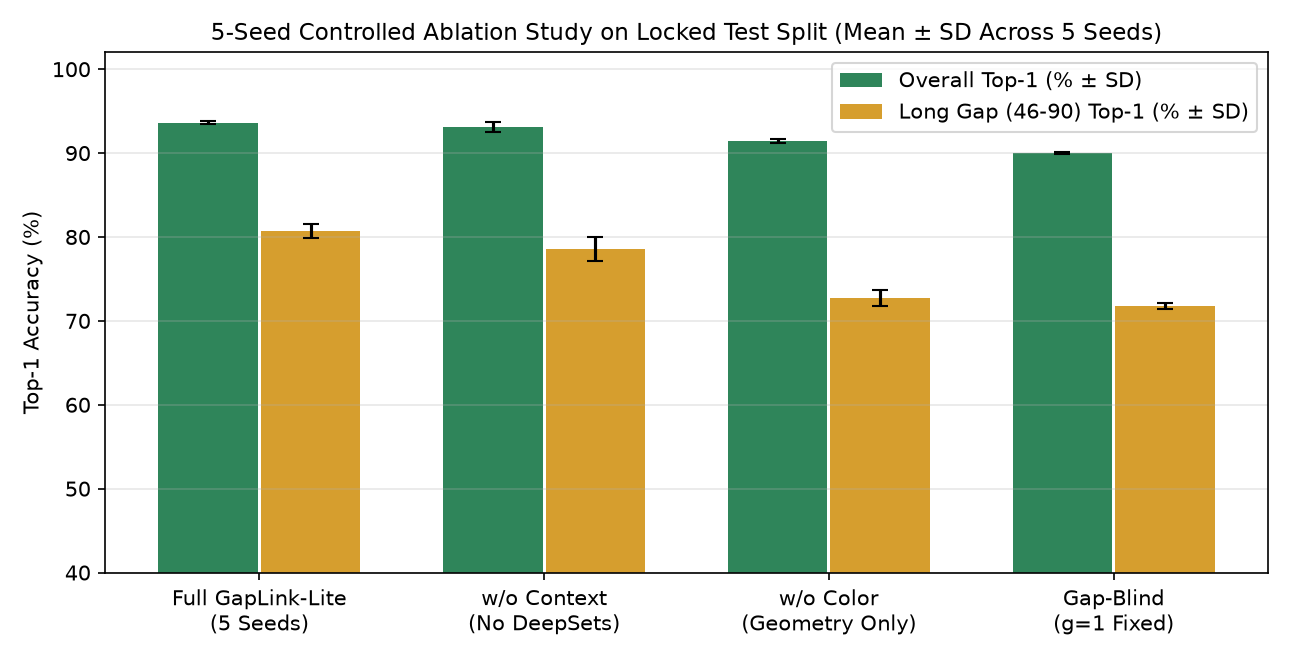
\includegraphics[width=0.88\textwidth]{figures/fig_ablation_study.png}
    \caption{5-Seed Ablation Study on Locked Test Events (Mean $\pm$ SD Across 5 Random Seeds)}
    \label{fig:ablation_plot}
\end{figure}

\textbf{Robustness.} Table~\ref{tab:sensitivity} perturbs the test events. GapLink-Lite keeps a wrong-link rate below $6\%$ under up to $8\times$ positional jitter and $30\%$ missing true candidates, conditions under which C-3's wrong-link rate rises to $28$--$35\%$.

\begin{table}[htbp]
    \centering
    \caption{Extended sensitivity analysis on locked test split ($12{,}000$ events, Seed 1 vs.\ C-3)}
    \label{tab:sensitivity}
    \small
    \begin{tabularx}{\textwidth}{X c c c c}
        \toprule
        \textbf{Perturbation Setting} & \textbf{GapLink Top-1 (\%)} & \textbf{GapLink WLR (\%)} & \textbf{C-3 Top-1 (\%)} & \textbf{C-3 WLR (\%)} \\
        \midrule
        Nominal ($\sigma=0.05$, $M\le 10$) & \textbf{93.41} & \textbf{3.01} & 80.29 & 19.24 \\
        Position Jitter ($2\times\sigma=0.10$) & \textbf{93.23} & \textbf{3.04} & 79.97 & 19.48 \\
        Position Jitter ($4\times\sigma=0.20$) & \textbf{89.39} & \textbf{3.56} & 77.48 & 20.84 \\
        Extreme Jitter ($8\times\sigma=0.40$) & \textbf{69.82} & \textbf{5.63} & 64.66 & 27.86 \\
        Reduced Candidate Cap ($M\le 5$) & \textbf{94.35} & \textbf{1.57} & 83.99 & 15.18 \\
        True-Candidate Dropout ($15\%$) & \textbf{92.98} & \textbf{4.02} & 72.12 & 27.16 \\
        True-Candidate Dropout ($30\%$) & \textbf{92.29} & \textbf{5.25} & 64.21 & 34.96 \\
        \bottomrule
    \end{tabularx}
\end{table}

\textbf{Iterative improvements.} Two changes shaped the final system. (i) An audit of the first locked test run revealed a data-conversion error (ignore regions merged into a fake track) and a lost-track window shorter than the longest gap; both were fixed and the model was re-trained and re-frozen (\texttt{844fc391\ldots}). (ii) Phase~2 showed that a model trained only on ground-truth boxes links too eagerly on detector boxes; detector-aware fine-tuning (v1.3) halved the live wrong-link rate relative to the strongest baseline. The complete change log, including variants abandoned on validation, is kept in \texttt{docs/DEVIATIONS.md}.
